\documentclass[fontsize=14pt, paper=a4, pagesize, DIV=calc]{scrartcl}

\usepackage[T2A]{fontenc}
\usepackage[utf8]{inputenc}
\usepackage[russian]{babel}
\usepackage{color}
\usepackage{listings}
\usepackage{indentfirst} % Красная строка
\usepackage{setspace}
\usepackage{enumitem}
\usepackage{graphicx}
\usepackage{float}
\usepackage{paratype}

\setstretch{1.5}

\lstset{
  basicstyle=\linespread{.94}\ttfamily,
  columns=fixed,
  breaklines=true,
  postbreak=\mbox{\textcolor{red}{$\hookrightarrow$}\space},
  belowskip=1ex,
  abovecaptionskip=0em,
  belowcaptionskip=1ex,
  aboveskip=1em,
  numbers=left,
}

\renewcommand{\lstlistingname}{Листинг}
\renewcommand{\lstlistlistingname}{Список \lstlistingname ов}

\floatstyle{ruled}
\floatname{ListingEnv}{Листинг}
\newfloat{ListingEnv}{H}{lol}[section]

\def\code#1{\texttt{#1}}

\begin{document}

\begin{titlepage}

\centering

\vfill

МИНИСТЕРСТВО~ОБРАЗОВАНИЯ~И~НАУКИ~РФ

\vfill

Федеральное государственное автономное образовательное\\
учреждение высшего образования\\
ЮЖНЫЙ~ФЕДЕРАЛЬНЫЙ~УНИВЕРСИТЕТ

\vfill

Институт математики, механики и компьютерных наук\\
имени И.~И.~Воровича

\vfill

Направление подготовки\\
Фундаментальная информатика и информационные технологии

\vspace{2cm}

\textsf
{ИССЛЕДОВАНИЕ ДЕТАЛЕЙ РЕАЛИЗАЦИИ ОТЛАДЧИКА GHCI}

\vfill

Выпускная квалификационная работа

\vspace{2cm}

\raggedleft

Студента 4 курса\\
Д.~Ш.~Мирзоева

\vfill

Научный руководитель:\\
Старший преподаватель кафедры информатики и вычислительного эксперимента
Мехмата ЮФУ В.~Н.~Брагилевский

\vspace{2cm}

\raggedright

\noindent\begin{tabular}{ll}
\makebox[2.5in]{\hrulefill} & \makebox[2.5in]{\hrulefill}\\
оценка(рейтинг) & подпись руководителя\\
\end{tabular}

\vspace{2cm}

\centering

Ростов-на-Дону

2018

\end{titlepage}

\tableofcontents
\newpage

\section{Введение}

Отладка -- это процесс устранения ошибок в программе. Для его упрощения
разработчки используют специальные прогрммы-отладчики. Они обладают общирным
набором средств контроля за выполнением программы. 

Хотя все отладчики различаются с точки зрения функциональности, можно выявить
общие принципы работы, присущие большинству из них. К примеру, часто бывает
удобно остановить работу программы в месте предполагаемой ошибки и посмотреть
значения доступных в этот момент переменных. Кроме того, отладчики позволяют
выполнять программу ``шаг за шагом``, то есть выполнять каждый раз лишь одну
строку программы. Это помогает после остановки проследить изменение значений
переменных и саму последовательность выполнения инструкций.

В данной работе мы исследуем детали реализации отладчика языка Хаскель,
встроенного в интерпретатор GHCi. 

\section{Ленивость}

Особый интерес заключается в том, что Хаскель является языком программирования
с ленивой стратегией вычисления. Это означает, что порядок вычисления не задан
явно. Продемонстрируем эту особенность на двух примерах.

\begin{ListingEnv}
\caption{Делим два числа на Си}
\label{lst:divFooBarC}
\begin{lstlisting}[language=c]
int divFooBar(void) {
    int foo, bar;
    foo = ...;
    bar = ...;
    return foo / bar;
}
\end{lstlisting}
\end{ListingEnv}

В листинге \ref{lst:divFooBarC} приведён пример на языке Си. Последовательнось
выполнения \code{divFooBar} будет такой и только такой: сначала вычислится
значение \code{foo}, потом вычислится \code{bar}, потом вычислится результат.

\begin{ListingEnv}
\caption{Делим два числа на Хаскель}
\label{lst:divFooBarHaskell}
\begin{lstlisting}
divFooBar =
    let foo = ...
        bar = ...
    in foo `div` bar
\end{lstlisting}
\end{ListingEnv}

Код в листинге \ref{lst:divFooBarHaskell} делает то же самое. Разница
заключается в ленивости. Значения в Хаскель не вычисляются сразу. Вычисление
выражения начинается только в тот момент, когда понадобится его результат. В
связи с этим становится трудно сказать в каком порядке будет выполняться
программа. \code{foo} и \code{bar} могут быть вычислены в любом порядке.

По этой причине GHCi имеет сложное устройство и не похож на отладчики
традиционных языков программирования.

\section{GHCi}

GHCi -- это интерпретатор Хаскель кода. Он является частью GHC, компилятора
языка Хаскель. GHCi позволяет вычислять значения и интерпритировать код. Кроме
того, в его состав входит отладчик.

\subsection{Команды отладчика}

\begin{itemize}
\item \code{:break} устанавливает точку останова;
\item \code{:force} и \code{:print} показывают значение выражения. Разница между ними в
том, что \code{:force} принудительно вычисляет его значение, а \code{:print} нет.
\item \code{:history} последние выполненные шаги вычисления;
\item \code{:forward} и \code{:back} перемещаются по истории вперед и назад
соответственно;
\item \code{:trace} включает историю вычислений;
\item \code{:step} производит один шаг вычисления;
\item \code{:continue} продолжает выполнение вычисления после остановки.
\end{itemize}

\subsection{Пример работы с отладчиком GHCi}

Рассмотрим простую программу, осуществляющую сортировку списка целых чисел
алгоритмом бытрой сортировки.

\begin{ListingEnv}
\caption{main.hs}
\begin{lstlisting}
qsort [] = []
qsort (a:as) = qsort left ++ [a] ++ qsort right
 where 
  left  = filter (<=a) as
  right = filter (a<) as

main = print (qsort [8, 4, 0, 3, 1, 23, 11, 18])
\end{lstlisting}
\end{ListingEnv}

Загрузим её в интерпретатор.

\begin{ListingEnv}
\caption{}
\begin{lstlisting}
$ ghci main.hs
Ok, modules loaded: Main.
*Main>
\end{lstlisting}
\end{ListingEnv}

Теперь можно добавить точку останова. Сделаем это на второй части определения
\code{qsort}.

\begin{ListingEnv}
\caption{}
\begin{lstlisting}
*Main> :break 2
Breakpoint 0 activated at main.hs:2:16-47
\end{lstlisting}
\end{ListingEnv}

Команда \code{:break 2} устанавливает точку останова на строке 2 последнего
загруженного модуля. В нашем случае это \code{main.hs}. Она выбирает самое
левое полное подвыражение на этой строке(\code{qsort left ++ [a] ++ qsort
right}).

Теперь можно запустить программу.

\begin{ListingEnv}
\caption{}
\begin{lstlisting}
*Main> :main
Stopped in Main.qsort, main.hs:2:16-47
_result :: [Integer] = _
a :: Integer = 8
left :: [Integer] = _
right :: [Integer] = _
[main.hs:2:16-47] *Main> 
\end{lstlisting}
\end{ListingEnv}

Выполнение приостановлено на точке останова. Подсказка ввода изменилась,
демонстрируя, что мы остановились и где мы остановились:
\code{main.hs:2:16-47}. Помимо этого выводится список доступных переменных.
Здесь можно заметить специальную переменную \code{\_result}, которая связана с
результатов текущего выражения. Для отображения значения переменной есть
команда \code{:print}.

\begin{ListingEnv}
\caption{}
\begin{lstlisting}
[main.hs:2:16-47] *Main> :print left
left = (_t1::[Integer])
\end{lstlisting}
\end{ListingEnv}

Заметим, что \code{left} не был вычислен, поэтому в его отображении отсутствует
полный список значений. Можно потребовать его вычисления. Для этого существует
команда \code{:force}. 

\begin{ListingEnv}
\caption{}
\begin{lstlisting}
[main.hs:2:16-47] *Main> :force left
left = [4,0,3,1]
\end{lstlisting}
\end{ListingEnv}

Стоит отметить, что вычисление подвыражения может не завершаться или
завершаться с ошибкой даже в том случае, когда вычисление выражение целиком
завершается успешно. Рассмотрим пример.

\begin{ListingEnv}
\caption{main.hs}
\begin{lstlisting}
a = 0
b = 1 `div` a
foo = if a == 0 then 0 else b
\end{lstlisting}
\end{ListingEnv}

Результатом вычисления foo будет ноль, а вовсе не ошибка как можно подумать,
заметив деление на ноль в строке 2. Это происходит благодаря ленивой стратегии
вычисления. Значение \code{b} не вычисляется, потому что его результат
никогда не требуется. 

\subsection{История вычислений}

В традиционных отладчиках существует понятие стека вызова функций. После
остановки в некотором месте программы он помогает понять, откуда мы туда
пришли. 

Стек состоит из адресов возврата функций, которые вычисляются в данный момент,
в порядке обратном порядку их вызова. По нему можно перемещаться, выясняя
значения локальных переменных в этих функциях.

Похожий доступ к стеку можно получить и в Хаскель, но это требует компиляции с
опцией \code{-prof}, которая включает оснащение кода системой профилирования.
Такой режим компиляции несовместим с отладчиком. 

Существует альтернатива - история вычислений. Выражения в Хаскель вычисляются
по мере необходимости, поэтому важнее стека вызовов может оказаться именно
последовательность предпринятых шагов вычисления. Историю таких шагов можно
получить с помощью команд \code{:trace} и \code{:hist}. Рассмотрим пример.

\begin{ListingEnv}
\caption{}
\begin{lstlisting}
*Main> :list qsort
1  qsort [] = []
2  qsort (a:as) = qsort left ++ [a] ++ qsort right
*Main> :b 1
Breakpoint 0 activated at main.hs:1:12-13
\end{lstlisting}
\end{ListingEnv}

Запустим сортировку небольшого списка с трассировкой с помощью команды \code{:trace}.

\begin{ListingEnv}
\caption{}
\begin{lstlisting}
*Main> :trace qsort [3, 2, 1]
Stopped in Main.qsort, main.hs:1:12-13
_result :: [a] = _
\end{lstlisting}
\end{ListingEnv}

Теперь мы можем посмотреть историю шагов вычисления. Для этого есть команда
\code{:hist}.

\begin{ListingEnv}
\caption{}
\begin{lstlisting}
[main.hs:1:12-13] *Main> :hist
-1  : qsort:left (main.hs:4:12-26)
-2  : qsort (main.hs:2:16-25)
-3  : qsort (main.hs:2:16-47)
-4  : qsort:left (main.hs:4:12-26)
-5  : qsort (main.hs:2:16-25)
-6  : qsort (main.hs:2:16-47)
-7  : qsort:left (main.hs:4:12-26)
-8  : qsort (main.hs:2:16-25)
-9  : qsort (main.hs:2:16-47)
<end of history> 
\end{lstlisting}
\end{ListingEnv}

Для перемещения по истории используются команды \code{:forward} и
\code{:backward}. Следом удобно использовать команду \code{:list}, которая
отображает исходный код места, на котором мы остановились и выделяет 
вычисляемое выражение.

\begin{ListingEnv}
\caption{}
\begin{lstlisting}
[main.hs:1:12-13] *Main> :back
Logged breakpoint at main.hs:4:12-26
_result :: [Integer]
a :: Integer
as :: [Integer]
[-1: main.hs:4:12-26] *Main> :list
3   where
4     left  = >>> filter (<=a) as <<<
5     right = filter (a<) as
[-1: main.hs:4:12-26] *Main> :forward
Stopped at main.hs:1:12-13
_result :: [a]
[main.hs:1:12-13] *Main> :list
1  qsort [] = >>> [] <<<
2  qsort (a:as) = qsort left ++ [a] ++ qsort right
\end{lstlisting}
\end{ListingEnv}

\section{Компиляция}

\begin{figure}[H]
\centering
\caption{Схема процесса компиляции}
\label{fig:compilation}
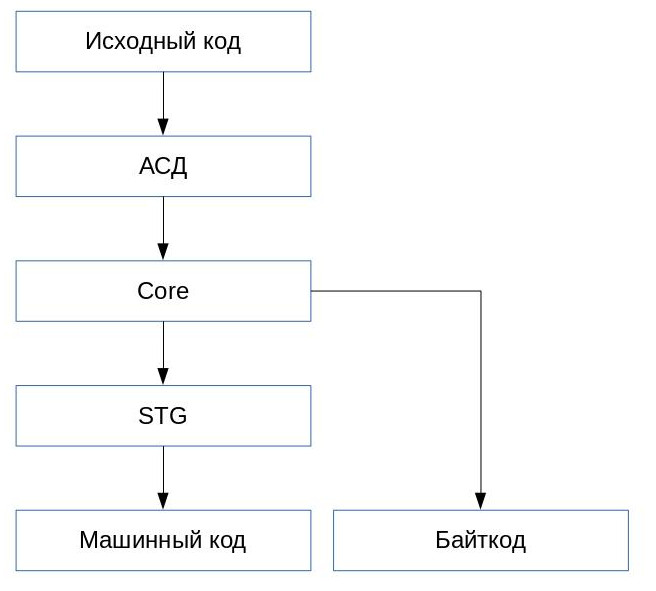
\includegraphics[scale=0.8]{compilation.jpg}
\end{figure}

На рисунке \ref{fig:compilation} приведена схема процесса компиляции.
Рассмотрим её более подробно. В прямоугольниках обозначена форма представления
программы на текущем этапе.

\subsection{Машинный код}

При компиляции отдельного файла на выходе получается исполняемый или объектный
файл, то есть машинный код. 

На вход компилятору поступает файл с исходным кодом. Он рассматривается как 
последовательность символов.

Эту последовательность символов обрабатывает лексический анализатор Alex и
превращает её в последовательность лексем. Последовательность лексем
обрабатывает синтаксический анализатор Happy и превращает её в абстрактное
синтаксическое дерево. Следом происходит проверка типов.

Следующий этап -- удаление синтаксического сахара. Хаскель транслируется в
промежуточный язык Core. Он имеет гораздо более простой синтаксис. На следующем
шаге происходят многочисленные оптимизации. Использование компактного
промежуточного языка позволяет упростить код связанный с оптимизацией и сделать
его в некоторой мере независимым от синтаксиса самого языка.

Последний шаг -- кодогенерация. Прежде всего Core транслируется в язык STG.
STG код транслируется в C-{}-. Это низкоуровневый императивный язык, который
используется в качестве переносимого ассемблера. Он может быть скомпилирован
напрямую в машинный код, а может быть транслирован в ещё одно промежуточное
представление: llvm или C. Это обеспечивает более высокий уровень оптимизации.

\subsubsection{Немного об STG}

STG это абстрактная машина для свёртки графов. Она была разработана специально
для компиляции функциональных языков в низкоуровневое машинное представление.
STG язык -- это язык команд этой машины. Он оперирует понятиями, которые легко
отобразить на существующие процессоры. Среди них стек, куча, регистры. 

STG расшифровывается как Spineless Tagless G-machine.

\begin{itemize}

\item \textbf{Spineless} означает, что у этой машины отсутствует spine. Spine -- это стек
укзазателей на самые левые узлы дерева.

\begin{figure}[H]
\centering
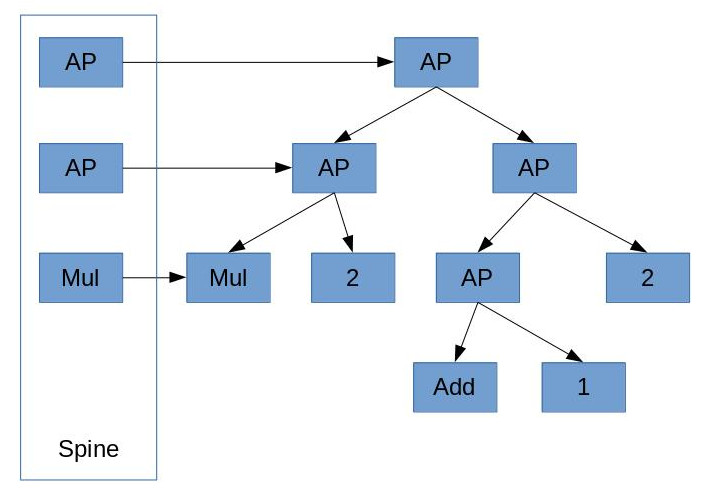
\includegraphics[scale=0.7]{spine.jpg}
\end{figure}

\item Структура объектов, которыми оперирует STG, похожа. Все они имеют первым
полем указатель на код, который нужно выполнить, чтобы вычислить их значение.
Поэтому для вычисления значения не нужно знать его точный тип. В структуре
объектов отсутствует поле, обозначающее тип, то есть tag. Отсюда \textbf{tagless} в
названии.

\item \textbf{G-machine} означает, что это машина для свёртки графов.

\end{itemize}

\subsection{Байткод}

Интерпретатор использует другой выходной формат. На выходе от компилятора он
требует Byte Code Object(BCO). В отличие от стандартной кодогенерации, входом
которой служит код С-{}-, входом генератора байткода служит Core.

\begin{ListingEnv}
\caption{compiler/llvm/LlvmCodeGen.hs}
\begin{lstlisting}[firstnumber=44]
llvmCodeGen :: DynFlags -> Handle -> UniqSupply
               -> Stream.Stream IO RawCmmGroup ()
               -> IO ()
\end{lstlisting}
\end{ListingEnv}

\begin{ListingEnv}
\caption{compiler/nativeGen/AsmCodeGen.hs}
\begin{lstlisting}[firstnumber=108]
nativeCodeGen :: DynFlags -> Module -> ModLocation -> Handle -> UniqSupply
              -> Stream IO RawCmmGroup ()
              -> IO UniqSupply
\end{lstlisting}
\end{ListingEnv}

\begin{ListingEnv}
\caption{compiler/ghci/ByteCodeGen.hs}
\begin{lstlisting}[firstnumber=81]
byteCodeGen :: HscEnv
            -> Module
            -> CoreProgram
            -> [TyCon]
            -> Maybe ModBreaks
            -> IO CompiledByteCode
\end{lstlisting}
\end{ListingEnv}

\code{BCO} -- это один из объектов, которыми оперирует STG. Они представляют из
себя массив инструкций байткода. Интерпретацией этих объектов занимется среда
времени выполнения. Интерпретатор во время своей работы взяимодействует со
средой выполнения, для исполнения своих команд.

\begin{ListingEnv}
\caption{rts/Interpreter.c}
\begin{lstlisting}[firstnumber=295]
Capability *
interpretBCO (Capability* cap)
{
\end{lstlisting}
\end{ListingEnv}

[1] Implementing lazy functional languages on stock hardware:
the Spineless Tagless G-machine, 1992, Simon L Peyton Jones

\end{document}
